\documentclass[11pt]{article}
\usepackage{geometry}
\geometry{margin=1in}
\usepackage{graphicx}
\usepackage{tikz}
\usetikzlibrary{shapes.geometric, arrows.meta}
\usepackage{enumitem}
\usepackage{hyperref}
\usepackage{xcolor}
\usepackage{booktabs}
\usepackage{fancyhdr}

% ---------- Handy macro for quick image placeholders ----------
\newcommand{\imageplaceholder}[2][]{%
  \begin{figure}[h]%
    \centering
    % Replace the box below with \includegraphics once the file is available
    \fbox{\rule{0pt}{2in}\rule{0.9\linewidth}{0pt}}%
    \caption{#2}%
    \label{fig:#1}%
  \end{figure}%
}

\pagestyle{fancy}
\fancyhead[L]{Sustainable Garden Rainwater System}
\fancyhead[R]{Troubleshooting Guide}
\fancyfoot[C]{\thepage}

\begin{document}

\begin{center}
  {\LARGE \textbf{Troubleshooting Guide for Rainwater Pumping System}}\\[1em]
  {\large \textit{Keep this guide posted by the control panel and review annually before the growing season.}}\\[2em]
\end{center}

\vspace{1em}

The product developed for the Sustainable Garden at Green Quad employs a dual–mode rain‑water irrigation system:
\begin{itemize}
  \item \textbf{Passive gravity‑fed system} – zero‑energy backup that delivers up to \(\sim20\;\text{gpm}\) when the tank is full.
  \item \textbf{Pressurized (active) system} – solar‑powered pump maintains \(20–40\;\text{psi}\) for sprinklers, with AC mains as a fallback.
\end{itemize}

This guide lists common failure modes, quick‑check steps, corrective actions, and preventive maintenance for the electrical, plumbing, and control subsystems.

%--------------------------------------------------
\section{System Overview Diagrams}
\subsection{High‑Level Layout}
\begin{figure}[h]
  \centering
  
\includegraphics[width=\linewidth]{Work_Products/overall.png}
  \caption{Overall view of entire system}
  \label{fig:overall}
\end{figure}


\newpage
\subsection{Electrical Block Diagram}
\begin{figure}[h]
  \centering
  
\includegraphics[width=\linewidth]{Work_Products/electrical.png}
  \caption{Diagram of solar panels, charge controller, battery, inverter, and 120 V branch.}
  \label{fig:electrical}
\end{figure}


\subsection{Plumbing Block Diagram}
\begin{figure}[h]
  \centering
  
\includegraphics[width=\linewidth]{Work_Products/plumbing.png}
  \caption{Diagram from 2 inch main through passive tee, pump, unions, check valve, pressure tank, and spigots.}
  \label{fig:plumbing}
\end{figure}

%--------------------------------------------------
\newpage\section*{Quick Check Flowchart}
\begin{figure}[h!]
  \centering
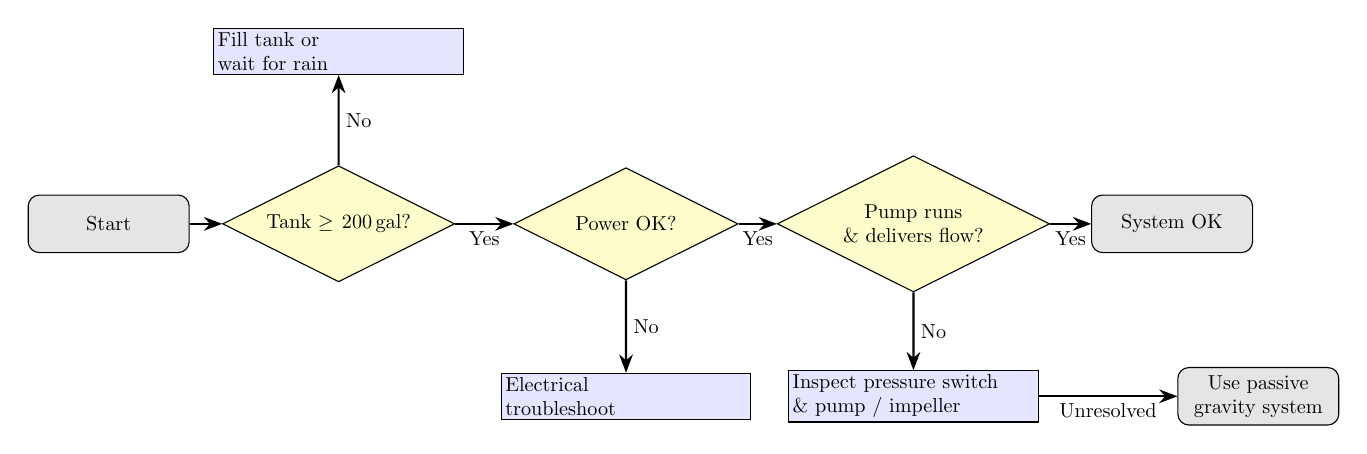
\begin{tikzpicture}[
    scale=0.73,           % global scale factor
    transform shape, 
    >=Stealth,
    startstop/.style = {
        rectangle, rounded corners,
        minimum width = 2.8cm, minimum height = 1cm,
        draw, fill = gray!20, align = center
    },
    decision/.style = {
        diamond, aspect = 2,
        text width = 3.2cm, align = center,
        draw, fill = yellow!20, inner sep = 1pt
    },
    process/.style = {
        rectangle, text width = 4.2cm, align = left,
        draw, fill = blue!10, inner sep = 2pt
    },
    arrow/.style = {thick, ->}
]

% --- Nodes placed by absolute coordinates (cm) ---
\node[startstop] (start)   at ( 0,  0)  {Start};

\node[decision] (tank)     at ( 4,  0)  {Tank $\ge{}200$\,gal?};

\node[process]  (fill)     at ( 4,  3)  {Fill tank or\\wait for rain};

\node[decision] (power)    at ( 9,  0)  {Power OK?};

\node[process]  (elec)     at ( 9, -3)  {Electrical\\troubleshoot};

\node[decision] (pump)     at (14,  0)  {Pump runs \\ \& delivers flow?};

\node[process]  (inspect)  at (14, -3)  {Inspect pressure switch\\\& pump / impeller};

\node[startstop] (success) at (18.5,  0)  {System OK};

\node[startstop] (passive) at (20, -3)  {Use passive\\gravity system};

% --- Arrows and labels ---
\draw[arrow] (start) -- (tank);

\draw[arrow] (tank)  -- node[below]{Yes} (power);
\draw[arrow] (tank)  -- node[right]{No}  (fill);

\draw[arrow] (power) -- node[below]{Yes} (pump);
\draw[arrow] (power) -- node[right]{No}  (elec);

\draw[arrow] (pump)  -- node[below]{Yes} (success);
\draw[arrow] (pump)  -- node[right]{No}  (inspect);

\draw[arrow] (inspect) -- node[below]{Unresolved} (passive);

\end{tikzpicture}
  \caption{Overall Quick Start Decision Flow}
  \label{fig:flowchart}
\end{figure}

\noindent Follow the numbered checks in order:
\begin{enumerate}[label=\arabic*.]
  \item \textbf{No/Low Water Output?} --- Go to \emph{Step 1: Main Valve \& Tank Check}
  \item \textbf{Active (Pressurized) System Failure?} --- Go to \emph{Step 2: Electrical \& Power Checks}
  \item \textbf{Pump Running but No Flow?} --- Go to \emph{Step 3: Pressure Switch \& Pump Inspection}
  \item \textbf{All Else Fails \textrightarrow Passive Backup} --- Go to \emph{Step 4: Passive Watering System}
\end{enumerate}

\section{Step 1: Main Valve \& Tank Check}
\begin{enumerate}[label=\arabic*.]
  \item Confirm Main Valve is \textbf{Fully Open}: see Fig.~\ref{fig:main-valve}.
  \begin{figure}[h!]
    \centering
    
\includegraphics[width=0.75\linewidth]{Work_Products/main_valve.png}
    \caption{Main Valve Detail}
    \label{fig:main-valve}
  \end{figure}
  \item Measure rainwater tank level:
    \begin{itemize}[leftmargin=*]
      \item \(<\!40\) gal \textemdash{} System OFF (cannot operate)
      \item 40--100 gal \textemdash{} LWD trips, system shuts off
      \item 100--200 gal \textemdash{} Pressurized flow only; passive mode unavailable
      \item \(>200\) gal \textemdash{} OK for both systems
    \end{itemize}
  \item If level \(<200\) gal:
    \begin{itemize}[leftmargin=*]
      \item Fill tank from city water spigot OR wait for rain.
    \end{itemize}
  \item Re-test flow. If still no/low output, proceed to \emph{Step 2}.
\end{enumerate}

\section{Step 2: Electrical \& Power Checks}

\subsection*{2.1 Inverter Status}
\begin{enumerate}[label=\arabic*.]
  \item Is the inverter switch ON? Is the \textcolor{green}{green LED} lit?
  \item If \textcolor{red}{no}: indicates inverter failure, loose wiring, or low battery. Perform:
    \begin{enumerate}[label=\alph*.]
      \item Turn inverter OFF.
      \item Inspect all screw terminal wire connections; tighten any loose.
      \item Turn inverter ON; check LED again.
    \end{enumerate}
  \begin{figure}[h!]
    \centering
    
\includegraphics[width=0.55\linewidth]{Work_Products/inverter.png}
    \caption{Inverter Control Panel}
    \label{fig:inverter-ctrl}
  \end{figure}
\end{enumerate}

\subsection*{2.2 Battery Voltage}
\begin{enumerate}[label=\arabic*.]
  \item Measure across battery terminals with a multimeter.
  \item If voltage \(<11.7\) V: battery too low, inverter won\textquotesingle t run.
    \begin{itemize}[leftmargin=*]
      \item Disconnect battery (red then black wires).
      \item Charge with car battery charger until \(\ge12.8\) V.
      \item If it won\textquotesingle t hold \(\ge12.8\) V: Replace battery.
    \end{itemize}
  \item If voltage OK but not rising, proceed to \emph{2.3 Charge Controller}.
    \begin{figure}[h!]
      \centering
        
\includegraphics[width=0.8\linewidth]{Work_Products/battery.png}
      \caption{Battery. Connect the black cables first, then red. Expect a small spark when first connecting red.}
      \label{fig:battery}
    \end{figure}
\end{enumerate}

\subsection*{2.3 Charge Controller \& Solar Panels}
\begin{enumerate}[label=\arabic*.]
  \item Is controller display active?
    \begin{itemize}[leftmargin=*]
      \item \textcolor{red}{No}: controller failure or panel wiring issue.
      \item \textcolor{green}{Yes}: verify “Solar $\to$ Battery” current reading.
    \end{itemize}
    \begin{figure}[h!]
      \centering
        
\includegraphics[width=0.55\linewidth]{Work_Products/Charge_controller.png}
      \caption{Charge Controller. Note the small cover at bottom needs to be removed for access.}
      \label{fig:charge-controller}
    \end{figure}
  \item If no solar voltage at controller input:
    \begin{itemize}[leftmargin=*]
      \item Disconnect each panel; test output in sunlight (should read $\sim12$ V).
      \item Any panel $<12$ V: Replace panel.
      \item Otherwise: re-terminate connectors or replace charge controller.
    \end{itemize}
\end{enumerate}

\vspace{0.5em}
\noindent\textbf{Note:} If inverter now powers pump but flow is low, skip Step~3 and retest. If inverter still won\textquotesingle t run, replace inverter (mains power can be used if inverter fails).

\section{Step 3: Pressure Switch \& Pump Inspection}
\begin{enumerate}[label=\arabic*.]
  \item \textbf{Bypass LWD:}
    \begin{itemize}[leftmargin=*]
      \item Plug pump directly into inverter’s 120 V outlet.
      \item Does pump run?
        \begin{itemize}[leftmargin=1.5em]
          \item No: proceed to 3.2.
          \item Yes: issue is LWD or its wiring; inspect/replace LWD.
        \end{itemize}
    \end{itemize}
  \item \textbf{Pressure Switch Check}
    \begin{enumerate}[label=\alph*.]
        \item Unplug the pump; Open Pressure Switch casing; Plug pump back in.
        \item \textbf{Warning:} This procedure involves working with 120V AC electrical circuits. Contact with live electrical components can cause serious injury or death. 
           \begin{figure}[h!]
        \centering
        
\includegraphics[width=0.65\linewidth]{Work_Products/switch.png}
        \caption{Pressure Switch Schematic}
        \label{fig:pressure-switch}
      \end{figure}
      \item With multimeter, check for 120 V at switch input and output when pressure drops.
        \begin{itemize}[leftmargin=*]
          \item No voltage at any screw/terminal: inverter issue; replace inverter.
          \item If voltage at only one screw: Replace pressure switch or check for small debris in switch.
        \end{itemize}


    \end{enumerate}
  \item \textbf{Pump \& Debris Inspection}
    \begin{enumerate}[label=\alph*.]
      \item If switch is good but pump still silent or runs without flow:
        \begin{itemize}[leftmargin=*]
          \item Power off system.
          \item Remove pump from housing; inspect impeller for debris/damage.
          \item If clogged or damaged: Replace pump assembly.
          \item Reinstall and retest flow.
        \end{itemize}
    \end{enumerate}
\end{enumerate}

\section{Step 4: Passive Watering Backup}
\begin{enumerate}[label=\arabic*.]
  \item Open passive valve (brass with red handle); see Fig.~\ref{fig:passive-valve}.
    \begin{figure}[h!]
      \centering
        
\includegraphics[width=0.55\linewidth]{Work_Products/passive.png}
      \caption{Passive Watering Valve}
      \label{fig:passive-valve}
    \end{figure}
  \item Gravity flow rates:
    \begin{itemize}[leftmargin=*]
      \item \(\ge250\) gal: fills a watering can in ~30 s
      \item \(\ge900\) gal: up to 20 gpm possible
    \end{itemize}
  \item Shut off for repairs: Close passive valve to isolate system entirely.
\end{enumerate}

\newpage\section*{Appendix: System Layout \& Key Components}
\begin{itemize}[leftmargin=*]
  \item Solar Array $\to$ Charge Controller $\to$ Battery $\to$ Inverter $\to$ Pumps \& LWD
  \item Plumbing Tee $\to$ 2\,in branch $\to$ Passive Valve $\to$ Watering cans
  \item Plumbing Tee $\to$ 3/4\,in branch $\to$ Pump House $\to$ Check Valve $\to$ Pressure Tank (52 gal) $\to$ Gauge/Switch $\to$ Exterior Spigot
  \item Safety Features:
    \begin{itemize}[leftmargin=*]
      \item Pressure relief valve
      \item Low water cutoff (LWD)
      \item Overheat \& low voltage alarms on inverter
      \item Winterization drain \& spigot
      \item Tone emitter for fault alerts
    \end{itemize}
\end{itemize}

%--------------------------------------------------
\section*{Replacement Parts List}
\begin{itemize}
  \item (2) 100 W, 12 V monocrystalline panels, MC‑4 connectors
  \item (1) 20 A MPPT charge controller, IP65
  \item (1) 50 Ah AGM deep‑cycle battery, M8 terminals
  \item (1) 1500 GPH submersible pump, ¾″ NPT
  \item (2) ¾″ PVC union
  \item Misc. valve pack: brass ball (¾″), PVC slip (2″), check (¾″)
\end{itemize}

%--------------------------------------------------
\section*{Document Control}
\begin{itemize}
  \item Version 1.0 – May 5 2025 – Initial issue.
  \item Author: JC Vaught; William Wenzel; Tanner Harmon; Presston McConnell
\end{itemize}

\end{document}
